\chapter{Biomedical relation extraction}
\label{c5}

A vast amount of information is recorded electronically in natural language text containing knowledge about many concepts and their relationships.
However, from a computational point of view, this text is considered \textit{unstructured} because its information is not organized in strucured forms such as databases \parencite{mccallum2005a}.
The human manual action of reading and interpreting the text to populate and enrich databases, with information in a computer readable form, is time consuming and burdensome.
Besides, the abundant number of text documents\footnote{In the recent years, almost one million scientific publications have been indexed per year in \as{medline}, as illustrated in \Cref{fig:medline}.} makes the manual extraction process, for knowledge base population (\as{kbp}), an impractical task---\as{kbp} consists in augmenting a knowledge base with discovered new facts about entities from a large text corpus \parencite{balog2018a}.
Therefore, it is mandatory to develop automatic methods to efficiently and accurately identify relationships in \textit{unstructured text}, that can improve the quality and coverage of the databases, and match the continued growth of text knowledge sources \parencite{ohta1997a,temkin2003a}.
The computational task to address this problem is known as \textit{relation extraction}~(\as{re}) and it is a fundamental piece in text data mining pipelines, that consists in identifying relationships between entities recorded in \textit{unstructured text} \parencite{bach2007a,pawar2017b,liu2020c}.
Relation extraction is relevant to \as{kbp} since discovered relationships can be used to complete missing information in a knowledge base.
A reference example is the Stanford \as{kbp} system\footnote{\url{https://nlp.stanford.edu/projects/kbp/}} which uses a relation extraction system as its workhorse \parencite{surdeanu2012a,angeli2014a}.

Traditionally, the information to be extracted is usually limited to a particular domain with specific and pre-defined types of entities and relations---as \textcite{balog2018a} mentions, this paradigm may be referred to as \textit{closed} information extraction.
On the other hand, \textit{open} information extraction operates in a domain-independent manner and does not assume beforehand a particular set of entity and relation types \parencite{banko2007a,soderland2010a,balog2018a}.
In this chapter, we are interested in the former scenario, where a set of entity and relation classes, from a specialized domain, is known in advance.
Specifically, our work is focused on studying \as{re} methodologies to identify interactions between biomedical terms, such as chemicals and genes, in the life-sciences scientific literature.
The automatic extraction of this information assists expert curators, in maitaining biological databases updated, and alleviates the demand for their work \parencite{yeh2003a,cotton2007a,singhal2016a}.
These databases foster knowledge discovery, helping researchers to test different hypotheses and deduce new facts.
As an example, the extraction of relationships within the biomedical domain helps to gather evidence about diseases and adverse drug reactions \parencite{gonzalezhernandez2022a}.
For instance, studies have shown that patients with diabetes have an increased risk of developing Alzheimer disease, but the underlying biological mechanisms responsible for that correlation are not well understood \parencite{simsrobinson2010a}, and text mining--based tools can deliver key insights \parencite{saik2021a}.

Relation extraction can also boost applications such as question answering \parencite{wang2012a} and information retrieval \parencite{mcdonald2005a}.
Generally, it follows a \textit{named entity recognition} step where entity mentions are identified in the text and grounded to standardized ontologies or vocabularies if a normalization method is employed.
Although the \textit{normalization} task is often disregarded, considering a joint resolution for all the three tasks---entity recognition, entity normalization, and relation extraction---is more useful in a real-world scenario \parencite{yaseen2019a} since researchers benefit from these systems for their text mining tasks \parencite{kim2019a}.
\Cref{fig:re} illustrates the classical \as{re} pipeline.

% \FloatBarrier
\begin{figure}[!tb]
\begin{center}
\includegraphics[width=\textwidth]{img/re/v1/img.pdf}
\caption{Entity and relation extraction pipeline.}
\label{fig:re}
\end{center}
\end{figure}
% \FloatBarrier


This chapter is focused on biomedical relation extraction from the scientific literature.
We first give a brief overview of the development of the \as{re} task enumerating biomedical \as{nlp} worldwide challenges and shared-tasks, and describe commonly used datasets.
Then, we introduce a deep neural network model for identifying chemical--protein interactions in \as{pubmed} scientific abstracts.
Extensive experiments were performed to train the neural network under different configurations including model architecture, hyper-parameters, and training data.
Finally, we discuss the limitations of our method, perform a detailed error analysis, and offer viable future research directions.


\section{Background}

A major research effort that tackled the relation extraction task was the \as{ace} (Automatic Content Extration)\footnote{\url{https://www.ldc.upenn.edu/collaborations/past-projects/ace}} program conducted by the National Institute of Standards and Technology (\as{nist}) of the United States, and the Linguistic Data Consortium (\as{ldc}) at the University of Pennsylvania \parencite{doddington2004a}.
This challenge included the recognition of entities (such as persons, organizations, or geographical locations)  and relations (such as employment or affiliation between a person and an organization, or a location relationship) in English, Chinese, and Arabic texts.
The \as{ldc}'s \as{ace} annotators tagged broadcast transcripts, newswire, and newspaper data producing training and test sets for common research task evaluations.
The \as{ace} program succeeded the Message Understanding Conferences (\asp{muc}), that similarly addressed the extraction of information related to person and organization entities \parencite{sundheim1996a,grishman1996a}.
Initiated in 2008, the Text Analysis Conference (\as{tac})\footnote{\url{https://tac.nist.gov}} followed the \as{ace} research program consisting in a series of workshops for large-scale evaluation of \as{nlp} systems.
The first \as{tac} cycle addressed tasks such as question answering and summarization, but knowledge base population was the main task in later editions \parencite{ji2010a,ji2011b,ji2011a,ellis2012a,surdeanu2013a}.
The aforementioned challenges focused on the development of \as{nlp} systems for the general-domain, although in recent years \as{tac} has also been targeting biomedical information extraction tasks.
In 2017, \as{tac} organized a task for identifying adverse drug reactions (\asp{adr}) found in drug labels \parencite{roberts2017a}.
Following up, in the 2018 and 2019 editions, challenges for extracting drug--drug interactions (\asp{ddi}) from drug labels were conducted \parencite{demnerfushman2018a,goodwin2019a}.

Likewise, other biomedical text mining efforts, particularly for relation extraction, took place during the past years.
The \as{lll}05 (Learning Language in Logic 2005 workshop) challenge focused on extracting gene--protein interactions in biology abstracts from the \as{medline} bibliographic database \parencite{nedellec2005a}.

BioCreative~II introduced the protein--protein interaction (\as{ppi}) extraction task where protein interaction pairs had to be predicted from \as{pubmed} records \parencite{krallinger2007a,krallinger2008b}.
BioCreative~V proposed a challenge task for automatic extraction of chemical--disease relations (\asp{cdr}), from \as{pubmed} abstracts, which aimed to support biocuration, new drug discovery, and drug safety surveillance \parencite{wei2015a,wei2016a}.
BioCreative~VI addressed two relation extraction tasks, relevant for precision medicine, both using \as{pubmed} abstracts: (1) the aim of track~4 was to identify experimentally verified \asp{ppi} affected by genetic mutations \parencite{dogan2017a,dogan2019a}; and (2) track~5 promoted the development of systems for detecting relations between chemicals and \asp{gpro} (gene and protein related objects) \parencite{krallinger2017a}.
Similarly, built with experience from the past edition, BioCreative~VII prepared a challenge task for text mining chemical--protein interactions (\asp{cpi}) but used a higher number of \as{pubmed} records for training and evaluation, and considered the identification of more interaction types \parencite{miranda2021a}.

In 2010, \as{i2b2}\footnote{The \as{i2b2} (Informatics for Integrating Biology and the Bedside) \as{nlp} challenges for clinical data are now housed in the Department of Biomedical Informatics at Harvard Medical School as \as{n2c2} (National \as{nlp} Clinical Challenges).} partnered with \as{va} (Veterans Affairs) Salt Lake City Health Care System to promote a task for detecting relations between medical problems, tests, and treatments in patient clinical reports \parencite{uzuner2011a}.
Similar work had also focused on the extraction of disease--treatment semantic relations (\textit{cure}, \textit{prevent}, or \textit{side effect}) but using biomedical abstracts from the \as{medline} bibliographic database \parencite{rosario2004a,frunza2010a}.
The 2012 \as{i2b2} challenge focused on temporal relations between clinical events (problems, tests, or treatments) and temporal expressions (dates, times, or durations) documented in clinical discharge summaries \parencite{sun2013b}.
The 2018 \as{n2c2} shared task focused on the extraction of adverse drug events (\asp{ade}) from clinical records \parencite{henry2019a}.

The \as{bionlp} Shared Task (\as{bionlp}-ST) series started in 2009 toward fine-grained information extraction in the biomedical domain.
The first edition, based on the GENIA corpus \parencite{ohta2002a,kim2003a,kim2008a}, was focused on the extraction of molecular events involving proteins and genes \parencite{kim2009a,kim2011b}.
This task, then renamed \textit{Genia event extraction}, was hosted again in the second, third, and fourth editions of the \as{bionlp}-ST.
The 2011 edition aimed to evaluate generalization of the systems to full-text papers \parencite{kim2011c}, whereas in the 2013 and 2016 editions the task was extended toward knowledge base construction \parencite{kim2013a,kim2015a,kim2016c}.
The \textit{Bacteria Biotopes} task introduced in the \as{bionlp}-ST 2011 consisted in extracting bacteria localization events, identifying the habitats of bacteria, from textbook documents \parencite{bossy2011a,bossy2012a}.
Later editions refined this task by (1) considering a more comprehensive and fine-grained categorization (normalization) of the entity mentions and respective events to domain knowledge sources such as the \as{ncbi} (National Center for Biotechnology Information) taxonomy \parencite{federhen2012a} and the OntoBiotope ontology \parencite{nedellec2018a}, and (2) using scientific literature such as abstracts and full-text articles from the \as{pubmed} database \parencite{bossy2013a,deleger2016a,bossy2019a}.
Also, the \as{bionlp}-ST 2011 \parencite{kim2011a,pyysalo2012b} organized other information extraction challenges including (1) the \textit{Epigenetics and Post-translational Modifications} task which focused on events of epigenetics interest \parencite{ohta2011a}, (2) the \textit{Infectious Diseases} task targeting biomolecular mechanisms of infectious diseases \parencite{pyysalo2011a}, and (3) the \textit{Entity Relations} task concerning part-of relations between a gene or protein and an associated entity \parencite{pyysalo2011b}.
Likewise, the \as{bionlp}-ST 2013 \parencite{nedellec2013a,pyysalo2015a,bossy2015a} addressed other challenges including (1) the \textit{Cancer Genetics} task that focused on the extraction of events relevant to cancer \parencite{pyysalo2013b}, (2) the \textit{Pathway Curation} task concerning the extraction of biomolecular reactions for supporting the development of biomolecular pathway models \parencite{ohta2013a}, and (3) the \textit{Gene Regulation Ontology} and \textit{Genic Regulation Network} tasks which addressed the identification of events and relations relevant to gene regulation \parencite{kim2013b,bossy2013b}.
The \as{bionlp}-OST (Open Shared Task)\footnote{In 2019, the \as{bionlp}-OST was organized as a reformulation of the previous efforts around the \as{bionlp}-ST.} 2019 also organized an extraction task addressing mutation--disease relationships to support knowledge discovery for drug repurposing \parencite{wang2019e}.

The SemEval-2013 Task 9, DDIExtraction 2013, evaluated the extraction of drug--drug interactions from biomedical texts \parencite{segurabedmar2013a} which followed the DDIExtraction-2011 challenge task \parencite{segurabedmar2011b}.

Much of the past work on biomedical information extraction relied on hand-labeled data to enable automatic training of machine learning models in a supervised fashion, but the manual annotation of ground-truth information, such as entity mentions and their interactions, in text documents is a labored and expensive task requiring expert professionals \parencite{baumgartner2007a,howe2008a,winnenburg2008a,karp2016a}.
Knowledge-based, unsupervised, and semi-supervised approaches aim to counteract the need of gold-standard data in developing competitive relation extraction systems.
These type of techniques have also been addressed in past work.
For instance, \textcite{craven1999a} present a distant supervision approach to extract information from text using knowledge bases, where they train classifiers using \textit{weakly labeled} training data.
The authors observed that for many information extraction tasks there are external knowledge sources that could be coupled with documents to create what they called \textit{weakly labeled} training examples.
They coined the term ``weak'' because each training instance does not consist of a precise annotated document, but rather it consists of a known fact---from a knowlege base---that may be asserted in a particular document.

Another example is the work of \textcite{mintz2009a} that continued to investigate the \textit{distant supervision} mechanism to create \textit{weakly labeled} data  of any size.
The authors relied on Freebase, a large semantic database, containing thousands of relationships \parencite{bollacker2008a}.
For every pair of entities present in the database, the authors found all sentences that contained those entities in an unlabeled corpus, and used these to train a relation classifier.
Distant supervision is now a mature technique and has been widely used in relation extraction systems that can benefit from knowledge bases as a source of training data \parencite{smirnova2019a}.

Early work on biomedical relation extraction focused on protein--protein interactions \parencite{blaschke1999a} and relationships betweens genes and drugs relevant to cancer \parencite{rindflesch1999a}.
\textcite{temkin2003a} proposed a system for extracting protein interaction information from unstructured text.
Their approach is based on an external database containing ditictionaries that are then used by a lexical analyzer followed by a parser, constructed around a context-free grammar \parencite{chomsky1956a,aho2007a}, that identifies interactions based on the rules of the grammar.
The rules of the context-free grammar were manually derived from 500 \as{pubmed} abstracts, whereas their final system was evaluated using a test corpus of 100 \as{pubmed} abstracts.

\textcite{airola2008a} propose a graph kernel--based approach for \as{ppi} extraction.
They assessed their method on five \as{ppi} annotated datasets, which as the authors state, provided the most comprehensive evaluation for a machine learning--based \as{ppi}-extraction system, and achieved a 0.564 F-score.
The authors performed cross-corpus evaluation for understanding how a trained model on a specific dataset with its own characteristics generalizes to a different dataset.
They also emphasize that the comparison of \as{re} systems must be done carefully because the use of different evaluation strategies and resources make results incomparable.

Previous research on biomedical relation extraction have been focusing on protein--protein interactions \parencite{krallinger2011a} and relations between drugs, genes and diseases \parencite{frijters2010a,krallinger2017b}.
Machine learning methods combined with kernel functions to calculate similarities between instances given some representation, were shown to achieve good results in textual relation extraction.

As opposed to the traditional machine learning methods employed in initial works, deep learning techniques eliminate the need for feature engineering, instead using multiple data transformation layers that apply simple non-linear functions to obtain different levels of representation of the input data, intrinsically learning complex classification functions \parencite{lecun2015a}.
These strengths have brought much attention with significant successes in \as{nlp} tasks, including word sense disambiguation \parencite{jimenoyepes2017a}, text classification \parencite{kim2014a,kowsari2017a}, and named entity recognition \parencite{habibi2017a,lyu2017a}.

Several works have demonstrated the use of deep neural networks for biomedical relation extraction and classification.
For example, \textcite{nguyen2015a} used a \as{cnn} (convolutional neural network) with pre-trained word embeddings, outperforming previous state-of-the-art systems for relation classification.
Nonetheless, the sequential nature of natural texts can be better modeled by recurrent networks, which contain a feedback loop that allows the network to use information regarding the previous state.
\as{lstm} (long short-term memory) networks are a special type of recurrent neural networks (\asp{rnn}) in which a set of information gates is introduced in the processing unit that allow these networks to memorize long-term dependencies while avoiding the vanishing gradient problem.
\textcite{wang2017a} used \as{bilstm} (bidirectional \as{lstm}) networks and features from the dependency structure of the sentences obtaining an F1-score of 0.720 in the DDIExtraction 2013 corpus.
\textcite{zhang2017a} also used \as{bilstm} models for extracting drug--drug interactions (\asp{ddi}) achieving a state-of-the-art F1-score of 0.729 in the same dataset.
They integrated the shortest dependency path (\as{sdp}) and sentence sequences, and concatenated word, part-of-speech and position embeddings into a unique embedding, and an attention mechanism was employed to give more weight to more relevant words.

Methods for extracting chemical-disease relations were evaluated in the BioCreative~V \as{cdr} task, in which participants were required to identify disease and chemical entities and relations between them \parencite{wei2016a}.
Using the provided gold-standard entities, \textcite{zhou2016a} achieved an F1-score of 0.560 with a hybrid system consisting of a feature-based \as{svm} (support vector machine) model, a tree kernel-based model using dependency features and a \as{lstm} network to generate semantic representations.
This result was improved to 0.613 by inclusion of post-processing rules.
The same result was achieved by \textcite{gu2017a}, also with an hybrid system combining a maximum entropy model with linguistic features, a \as{cnn} using dependency parsing information, and heuristic rules.

Regarding chemical--protein relation extraction, the state-of-the-art results were achieved by teams participating in the BioCreative~VI ChemProt challenge \parencite{krallinger2017a}, with some improvements described in follow-up works.
The best participating team achieved an F1-score of 0.641 using a stacking ensemble combining a \as{svm}, a \as{cnn}, and a \as{bilstm} \parencite{peng2017b,peng2018a}.
Lemmatization, \as{pos} (part-of-speech), and chunk labels from the surrounding entity mentions and from the shortest dependency path were used as features for the \as{svm} classifier.
For the \as{cnn} and \as{bilstm}, the sentence and shortest path sequences were used, where each word was represented by a concatenation of several embeddings (\as{pos} tags, dependencies, named entities, and others).
\textcite{corbett2017a} achieved an F1-score of 0.614 using pre-trained word embeddings and a network model with multiple \as{lstm} layers, with the ChemListem \as{ner} system used for tokenization \parencite{corbett2017b}.
This result was improved to an F1-score of 0.626 in post-challenge experiments \parencite{corbett2018a}.
\textcite{mehryary2017a} proposed two different systems: a \as{svm} classifier and an ensemble of neural networks that use \as{lstm} layers.
Both systems took features from the dependency parsing graph, although the \as{svm} required more feature engineering.
They combined the predictions of the two systems, yet the \as{svm} alone produced the best F1-score (0.610).
After the challenge they achieved an F1-score of 0.631 by using their improved artificial neural network (\as{ann}) \parencite{mehryary2018a}.
\textcite{lim2017a} used ensembles of tree-\as{lstm} networks, achieving an F-score of 0.585 during the challenge.
They later improved this result to 0.637 with a revised pre-processing and by using more members in the ensemble, and equaled the best challenge F1-score (0.641) using a shift-reduce parser based network architecture \parencite{lim2018a}.
\textcite{lung2017a,lung2019a} achieved an F1-score of 0.567 using traditional machine learning.
Neural networks with attention mechanisms were also followed by \textcite{liu2017d,liu2018a,verga2017a}, but achieved lower results.
However, the use of attention layers \parencite{bahdanau2014a,vaswani2017a} has been shown to be effective in different information extraction tasks such as document classification \parencite{yang2016a} and relation extraction \parencite{shen2016a}, being an interesting direction to explore.

\textcite{zhang2019a} present a semi-supervised approach based on a variational autoencoder for biomedical relation extraction.
They evaluated their method in the ChemProt dataset experimenting with different number of labeled samples, showing that adding unlabeled data improves the relation extraction mainly when there are only a few hundred training samples.
Using 4000 (from a total of 25\,071) labeled training instances together with unlabeled data taken from the remaining training instances (with true labels removed), their semi-supervised method achieved an F-score of 0.509.

Lastly, a recent work by \textcite{zhang2019b} achieved the state-of-the-art F-score of 0.659 using \as{bilstm} models with deep context representation (providing superior sentence representation compared to traditional word embeddings) and multi-head attention.

\textcite{huang2017a} used a support vector machine and \as{lstm} networks to identify drug--drug interactions, but most recent works often solely use neural networks.
For example, \textcite{asada2021a} used SciBERT---a tranformer model trained on biomedical text \parencite{beltagy2019c}---and external database information to boost \as{ddi} extraction performance.

For more information on related works and challenges about extracting relations from the biomedical literature we point the reader to major review works \parencite{hirschman2002a,krallinger2005a,ananiadou2006a,huang2016a,zhang2019j,zhao2021a}.
\textcite{zhang2019j} present an extensive review of neural network--based approaches for biomedical \as{re} classification.
They discuss works identifying \asp{ppi} and \asp{ddi} in the biomedical literature, and methods including \asp{cnn} and \asp{rnn}.
They present several corpora, and discuss different word embeddings models.
Finally, they detail current challenges and present potential directions to further improve the performance of the biomedical \as{re} task.

Regarding the availability of high-quality datasets for assessing the performance of biomedical relation extraction systems many corpora have been manually annotated over the past years (\Cref{tab:re-datasets}).
Some of these were developed for worldwide challenges and shared-tasks whereas others were published by particular research groups which allowed other researchers to assess and compare their methods with previous results.

\begingroup
\normalfont
\color{black}
\singlespacing

\newcommand{\z}{\hspace*{0.5em}}
\newcommand{\minorsmall}{\fontsize{10.0pt}{12.0pt}\selectfont}
% \newcommand{\minorsmall}{\fontsize{10.5pt}{12.6pt}\selectfont}
% \newcommand{\minorfootnotesize}{\fontsize{9.7pt}{11.64pt}\selectfont}

% https://tex.stackexchange.com/questions/446919/longtable-midrule-after-newpage

% \small

\begin{longtable}[c]{E{0.30\textwidth}p{0.62\textwidth}}%
\endfirsthead
\toprule
% \textbf{Resource} & \textbf{Description}\\
Resource & Description\\
\midrule
\endhead

\caption[Datasets for biomedical relation extraction.]{Datasets for biomedical relation extraction, presented in chronological order. ADE: adverse drug effect. CDR: chemical--disease relation. DDI: drug--drug interaction. IPS: interaction pair subtask. PPI: protein--protein interaction.}
\label{tab:re-datasets}\\

\toprule

% \textbf{Resource} & \textbf{Description}\\
Resource & Description\\

\midrule

BioText\newline
\z{\minorsmall\parencite{rosario2004a}}
&
This dataset concentrates on disease--treatment semantic relations (\textit{cure}, \textit{prevent}, or \textit{side effect}) using biomedical text found in the titles and abstracts from the \as{medline} 2001 database.
An annotator with a biological background performed the labeling.
\newline
{\footnotesize\url{https://biotext.berkeley.edu/data/dis_treat_data.html}}
\\

\midrule

AIMed\newline
\z{\minorsmall\parencite{bunescu2005b}}\newline
\z{\minorsmall\parencite{bunescu2005c}}\newline
\z{\minorsmall\parencite{bunescu2007a}}
&
The corpus is annotated with human protein names (genes and proteins are interchangeable) and their interactions.
It consists of 225 \as{medline} abstracts, containing 4084 protein mentions and around 1000 interactions.
\newline
{\footnotesize\url{https://www.cs.utexas.edu/ftp/mooney/bio-data/}}
\\

\midrule

BioInfer\newline
\z{\minorsmall\parencite{pyysalo2007a}}
&
The resource contains 1100 sentences from abstracts of biomedical research articles. These are annotated with named entities of the protein, gene, and \as{rna} types, their relationships, and syntactic dependencies. The corpus contains a total of 6349 entities and 2662 relationships.
% \newline
% {\footnotesize\url{https://bionlp.utu.fi/bioinfer.html}}
\\

\midrule

BioCreative~II PPI IPS\newline
\z{\minorsmall\parencite{krallinger2007a}}\newline
\z{\minorsmall\parencite{krallinger2008b}}
&
A corpus of full-text articles annotated with binary protein--protein interaction pairs. It is split into two sets: a \textit{training} collection of 740 articles and a smaller \textit{test} set of 358 articles.
\newline
{\footnotesize\url{http://biocreative.sourceforge.net/bc2_ppi_ips.html}}
\\

\midrule

2010 i2b2/VA Challenge\newline
\z{\minorsmall\parencite{uzuner2011a}}
&
A corpus of patient reports focused on medical concept extraction and relation classification between medical problems, tests, and treatments. It contains a total of 394 \textit{training} reports and 477 \textit{test} reports manually annotated.\newline
{\footnotesize\url{https://portal.dbmi.hms.harvard.edu/projects/n2c2-nlp/}}
\\

\midrule

ADE corpus\newline
\z{\minorsmall\parencite{gurulingappa2012a}}\newline
\z{\minorsmall\parencite{gurulingappa2012b}}
&
A corpus containing 2972 \as{medline} case reports annotated with two types of relations: drug-related adverse events (signs, symptoms, diseases, disorders, and others) and drug--dosage information (such as quantitative measurements or frequency mentions).\newline
{\footnotesize\url{https://sites.google.com/site/adecorpus/}}
\\

\midrule

DDI corpus\newline
\z{\minorsmall\parencite{herrerozazo2013a}}\newline
\z{\minorsmall\parencite{segurabedmar2013a}}\newline
\z{\minorsmall\parencite{segurabedmar2014a}}
&
A corpus containing 792 texts from the DrugBank database and other 233 \as{pubmed} abstracts. These are annotated with 18\,502 pharmacological substances and 5028 drug--drug interactions.\newline
{\footnotesize\url{https://github.com/isegura/DDICorpus}}
\\

\midrule

CDR corpus\newline
\z{\minorsmall\parencite{li2016b}}
&
A collection of 1500 \as{pubmed} abstracts manually annotated with 3116 chemical--disease relations and the respective named entities (4409 chemicals and 5818 diseases). The entity annotations also contain normalized \as{mesh} concept identifiers.\newline
{\footnotesize\url{https://biocreative.bioinformatics.udel.edu/tasks/biocreative-v/track-3-cdr/}}
\\

\midrule

ChemProt\newline
\z{\minorsmall\parencite{krallinger2017a}}
&
It contains a total of 2432 PubMed abstracts split into \textit{training}, \textit{development}, and \textit{test} subsets. With 31\,831 chemical and 30\,316 protein annotations, there are a total of 15\,739 chemical--protein interactions. Five different relation types are annotated: \textit{activation}, \textit{inhibition}, \textit{agonist}, \textit{antagonist}, and \textit{substrate}.\newline
{\footnotesize\url{https://biocreative.bioinformatics.udel.edu/tasks/biocreative-vi/track-5/}}
\\

\midrule

2018 n2c2 Track 2\newline
\z{\minorsmall\parencite{henry2019a}}
&
A collection of 505 narrative discharge summaries from the \as{mimic}-III clinical care database. These are annotated with concepts related to medications (strengths and dosages, duration and frequency of administration, route of administration, reason for administration, and adverse drug effects), and interactions between them. There are a total of 83\,869 named entities and 59\,810 relations.\newline
{\footnotesize\url{https://portal.dbmi.hms.harvard.edu/projects/n2c2-nlp/}}
\\

\midrule

DrugProt\newline
\z{\minorsmall\parencite{miranda2021a}}
&
Built from the existing ChemProt corpus, it includes more PubMed abstracts and is also split into three subsets (\textit{training}, \textit{development}, and \textit{test}). A total of 3500 documents with over 100 thousand annotated entities and interactions. Moreover, it contains more relation types---a total of 13 distinct chemical--protein interactions.\newline
{\footnotesize\url{https://biocreative.bioinformatics.udel.edu/tasks/biocreative-vii/track-1/}}
\\

\midrule

BioRED\newline
\z{\minorsmall\parencite{luo2022b}}
&
This corpus contains a set of 600 \as{pubmed} abstracts annotated with multiple entity types (genes, diseases, chemicals) and relation pairs (such as gene--disease and chemical--chemical). Each relation is further labeled as describing either a novel finding or background knowledge. It contains a total of 20\,419 entity mentions and 6503 relations.\newline
{\footnotesize\url{https://ftp.ncbi.nlm.nih.gov/pub/lu/BioRED/}}
\\

\midrule

ChemDisGene\newline
\z{\minorsmall\parencite{zhang2022b}}
&
A distant supervision corpus for extracting multi-class multi-label relations between chemicals, diseases, and genes. The dataset contains around 80 thousand \as{pubmed} abstracts and is split into two portions: (1) one curated by human experts intended for \textit{evaluation} containing 523 documents, and (2) another intended for \textit{training} which was distantly labeleled via the Comparative Toxicogenomics Database (\as{ctd}). The dataset is annotated with 18 relation types.\newline
{\footnotesize\url{https://github.com/chanzuckerberg/ChemDisGene}}
\\

\bottomrule

\end{longtable}
\endgroup



\section{Text mining chemical--protein interactions}

The scientific literature contains large amounts of information on genes, proteins, chemicals, and their interactions.
Extraction and integration of this information in curated knowledge bases helps researchers support their experimental results, leading to new hypotheses and discoveries.
This is especially relevant for precision medicine, which aims to understand the individual variability across patient groups in order to select the most appropriate treatments.
Methods for improved retrieval and automatic relation extraction from biomedical literature are therefore required for collecting structured information from the growing number of published works.

As the knowledge of how biological systems work at different structural levels grows, more possibilities arise for applying it in diagnosing and treating common and complex diseases.
Furthermore, exploiting the large amounts of biomolecular data from -omics studies and patient-level information recorded in electronic health records (\asp{ehr}) offers prospects for precision and personalized medicine \parencite{wu2017a}.
Nonetheless, relevant fine-grained information is constantly being communicated in the form of natural language through scientific publications.
To exploit this source of updated knowledge, several methods have been proposed for retrieving relevant articles for database curation \parencite{wang2016c}, and for extracting from the unstructured texts information such as entity mentions \parencite{campos2013b,nunes2013b}, biomolecular interactions and events \parencite{ananiadou2015a,krallinger2011a}, or the clinical and pharmacological impact of genetic mutations \parencite{singhal2016a}.
These methods have proven essential for collecting the most recent research results and for expediting database curation \parencite{krallinger2017b}.

The BioCreative~VI ChemProt challenge stimulated the development of systems for extracting interactions between chemical compounds (drugs) and \asp{gpro} (gene and protein related objects) from running text, given their importance for precision medicine, drug discovery and basic biomedical research \parencite{krallinger2017a}.
An example illustrating various relations that can be extracted from a single sentence in a publication is shown in \Cref{fig:chemprot-example-sentence}.
The development of systems able to automatically extract such relations may expedite curation work and contribute to the amount of information available in structured annotation databases, in a form that is easily searched and retrieved by researchers.

% \FloatBarrier
\begin{figure}[!tb]
\begin{center}
\includegraphics[width=\textwidth]{img/chemprot-example-sentence/v3/img.pdf}
\caption[Example sentence illustrating biochemical entities and their relations.]%
{Example sentence illustrating biochemical entities and their relations from the ChemProt training dataset (PMID 8667211).}
\label{fig:chemprot-example-sentence}
\end{center}
\end{figure}
% \FloatBarrier


Data for the ChemProt task was composed of PubMed abstracts in which gold-standard entities were provided, and the aim was to detect chemical--protein pairs that expressed a certain interaction.
Therefore, the biomedical named entity recognition step was out of the scope of this task.
The organizers defined ten groups of chemical--protein relations (\asp{cpr}) that shared some underlying biological properties, in which only five of them (up-regulation, down-regulation, agonist, antagonist, and substrate) were used for evaluation purposes.
More detail about the data is presented in \Cref{c5:ss:materials}.

In this section, we present a deep learning approach for extracting mentions of chemical--protein interactions from biomedical articles, based on various enhancements following our participation in the BioCreative~VI ChemProt task.
A significant aspect of our best method is the use of a simple deep learning model together with a very narrow representation of the relation instances, using only up to ten words from the shortest dependency path and the respective dependency edges.
\as{bilstm} recurrent networks or \asp{cnn} are used to build the deep learning models.

We report the results of several experiments and show that our best model is competitive with more complex sentence representations or network structures, achieving an F1-score of 0.6306 on the test set.
The source code of our work, along with detailed statistics, is publicly available at:

\centerline{\url{https://github.com/ruiantunes/biocreative-vi-track-5-chemprot}.}


\subsection{Materials and methods}
\label{c5:ss:materials}

This section describes the resources used, the evaluation metric employed, and the methods implemented.


\subsubsection{Dataset}

The ChemProt corpus was created by the BioCreative VI organizers \parencite{krallinger2017a}, being composed of three distinct sets: training, development, and test (\Cref{tab:chemprot-dataset}).
During the challenge, to hinder manual corrections and to ensure that systems could annotate larger datasets, the organizers included 2599 extra documents in the test set, which were not used for evaluation.

Each document, containing the title and the abstract of a PubMed article, was annotated by expert curators with chemical and protein entity mentions, and their relations.
The annotation guidelines considered ten groups of biological interactions, which were designated as chemical--protein relation groups.
However, for this task, only five classes were considered for evaluation purposes: activation (CPR:3), inhibition (CPR:4), agonist (CPR:5), antagonist (CPR:6), and substrate (CPR:9).
\Cref{tab:chemprot-dataset} presents detailed dataset statistics.

\begingroup
% \newcommand{\minorsmall}{\fontsize{10.5pt}{12.6pt}\selectfont}
% \renewcommand*{\arraystretch}{1.1}

\begin{table}[!t]

\centering

% \tiny
% \scriptsize
% \footnotesize
% \minorsmall
% \small

\caption[ChemProt dataset statistics.]{ChemProt dataset statistics.}
\label{tab:chemprot-dataset}

\begin{tabular}{D{19mm}D{20mm}D{13mm}G{17mm}G{26mm}G{15.5mm}}

\toprule

% & & & \textbf{Training} & \textbf{Development} & \textbf{Test}\\
& & & Training & Development & Test\\

\midrule

Abstracts & \multicolumn{2}{l}{Total}                    & 1020 & 612 & 800\\
          & \multicolumn{2}{l}{With any relation}        &  767 & 443 & 620\\
          & \multicolumn{2}{l}{With evaluated relations} &  635 & 376 & 514\\

\midrule

Entities & Chemical & & 13\,017 &    8004 & 10\,810\\
         & Protein  & & 12\,735 &    7563 & 10\,018\\
         & Total    & & 25\,752 & 15\,567 & 20\,828\\

\midrule

Relations & Activation & (CPR:3) &  768 &  550 &  665\\
          & Inhibition & (CPR:4) & 2254 & 1094 & 1661\\
          & Agonist    & (CPR:5) &  173 &  116 &  195\\
          & Antagonist & (CPR:6) &  235 &  199 &  293\\
          & Substrate  & (CPR:9) &  727 &  457 &  644\\
          & Total      &         & 6437 & 3558 & 5744\\

\bottomrule

\end{tabular}

\end{table}
\endgroup


One can see from \Cref{tab:chemprot-dataset} that not all abstracts contain annotated relations, although all abstracts were annotated with entity mentions.
Nevertheless, abstracts without evaluated relations are useful as they can be used to create negative instances for training the system.
Only 1525 documents of 2432 (63\%) are annotated with evaluated relations.
This suggests that it could be a reasonable idea to first apply a document triage step to ignore documents that probably are not relevant for extracting chemical--protein interactions, reducing the number of false positive relations, while still considering them for generating negative instances to feed the deep learning model.
Though, we did not follow this possibility leaving it as possible future work.
Similar binary approaches were followed by \textcite{lung2017a,lung2019a,warikoo2018a} who start by predicting if a CPR pair is positive.

A more scrupulous analysis of the corpus shows that there are some relations between overlapped entities (for example, a protein entity containing a chemical entity), as well as some cross-sentence relations.
However, cross-sentence relations appear in a very small number and were deliberately discarded.
Also, despite some ChemProt relations were classified with more than one CPR group we considered only one label, since these are rare, simplifying the task as a multi-class problem.


\subsubsection{Performance evaluation}

The BioCreative VI ChemProt organizers considered the micro-averaged precision, recall, and balanced micro F1-score for evaluation purposes \parencite{krallinger2017a}.
Micro F1-score was the official metric used to evaluate and compare the teams' submissions.
This metric was integrated in our pipeline, for measuring the neural network performance at each training epoch, allowing to develop and select the best model dynamically for this specific task.


\subsubsection{Pre-processing}

We pre-processed the entire ChemProt dataset using the Turku Event Extraction System (\as{tees}) \parencite{bjorne2015a} applying a pipeline composed with the GENIA sentence splitter \parencite{saetre2007a}, the \as{bllip} parser \parencite{charniak2005a} using the McClosky and Charniak (McCC) biomedical parsing model \parencite{mcclosky2008a}, and the Stanford dependency parser \parencite{chen2014a} (version 3.8.0, released on 2017-06-09).
This pre-processing performs sentence splitting, tokenization, part-of-speech tagging, and dependency parsing.
Sentence splitting is required to obtain all the chemical--protein pair candidates in the same sentence, since these are the only ones we considered.
The yielded tokens, PoS tags, and dependency labels are encoded using embedding vectors (more detail in the next sections).
The dependency parsing structure is also used to find the shortest dependency path between the two entities, since previous work had already proven its value for relation extraction \parencite{bunescu2005a}.

For every chemical--protein pair in each sentence, we obtain five sequences using the \as{tees} output: the SDP and the sequences containing the left text and the right text of the chemical and protein entities (\Cref{fig:chemprot-sdp}).
Like the work of \textcite{mehryary2017a,mehryary2018a}, our system traverses the shortest dependency path always from the chemical entity to the protein entity.
For entities spanning more than one word, we obtain the shortest path starting from the head word, as indicated by the \as{tees} result.
For each chemical--protein pair candidate instance, the chemical and protein entities (in cause) are replaced respectively by the placeholders `\#chemical' and `\#gene', except when the chemical--protein pair comes only from a single token (overlapped entities) which in this case is replaced by `\#chemical\#gene'.
While in the SDP the dependency features were obtained traversing the path, in the four left and right sequences the incoming edge of each token was used as dependency features.
If a token did not have an incoming edge or it was the last token in the SDP then the dependency feature was set to `\#none'.
Each one of the five sequences is therefore represented by a sequence of tokens, PoS tags, and dependency edge labels.

% References:
% https://nlp.stanford.edu/software/stanford-dependencies.shtml
% https://downloads.cs.stanford.edu/nlp/software/dependencies_manual.pdf
% https://www.ling.upenn.edu/courses/Fall_2003/ling001/penn_treebank_pos.html
% https://catalog.ldc.upenn.edu/docs/LDC95T7/cl93.html

\begin{figure}[!tb]
\centerline{\includegraphics[width=\textwidth]{img/chemprot-sdp/v2/img.pdf}}
\caption[Example illustrating the dependency parsing structure of a sentence.]%
{Example illustrating the dependency parsing structure of a sentence from the ChemProt training dataset (PMID 8667211). In this example, we considered the relation between the `acetazolamide' chemical mention and the `CA I' protein mention. The shortest dependency path is highlighted in bold. Penn Treebank part-of-speech tags \parencite{marcus1993a} used in this example: coordinating conjunction (CC); determiner (DT); preposition or subordinating conjunction (IN); adjective (JJ); noun, singular or mass (NN); verb, past tense (VBD); sentence final punctuation (.). Stanford dependencies \parencite{marneffe2016a} used in this example: adjectival modifier (amod); conjunction and (conj\_and); determiner (det); direct object (dobj); noun compound modifier (nn); nominal subject (nsubj); prepositional modifier of (prep\_of); prepositional modifier on (prep\_on); punctuation (punct).}
\label{fig:chemprot-sdp}
\end{figure}


Taking the sentence in \Cref{fig:chemprot-sdp} as example, and considering the chemical--protein pair [`acetazolamide', `CA I'], the five extracted sequences (containing the tokens, PoS tags, and dependency edges) are:

\begin{enumerate}
\item
\textbf{Shortest dependency path:} \#chemical / NN / prep\_of --- effect / NN / prep\_on --- \#gene / NN / \#none;
\item
\textbf{Chemical left text:} Indomethacin / NN / nsubj --- abolished / VBD / \#none --- the / DT / det --- inhibitory / JJ / amod --- effect / NN / dobj --- of / IN / \#none;
\item
\textbf{Chemical right text:} on / IN / \#none;
\item
\textbf{Protein left text:} in this case, it is the same as the chemical right text;
\item
\textbf{Protein right text:} and / CC / \#none --- CA / NN / nn --- II / NN / prep\_on --- . / . / punct.
\end{enumerate}

The SDP together with the left and right sequences are fed to the neural network through embedding layers, as explained in the following sections.


\subsubsection{Word embeddings}

For text based tasks, it is necessary to encode the input data in a way that it can be used by the deep network classifier.
This can be achieved by representing words as embedding vectors of a relatively small dimension, rather than using the large feature space resulting from the traditional one-hot encoding.
Word embeddings is a technique that consists in deriving vector representations of words, such that words with similar semantics are represented by vectors that are close to one another in the vector space \parencite{bengio2003a}.
This way, each document is represented by a sequence of word vectors which are fed directly to the network.
Efficient calculation of word embeddings, such as provided by word2vec \parencite{mikolov2013b}, allow inferring word representations from large unannotated corpora.

We applied the word2vec implementation from the Gensim framework \parencite{rehurek2010a} to obtain word embeddings from 15 million PubMed abstracts in English language from the years 1900 to 2015.
In previous research we created six models, with vector sizes of 100 and 300 features and windows of 5, 20, and 50.
The models contain around 775 thousand distinct words (stop words were removed).
These pre-trained word embeddings models showed their value achieving favorable results both in biomedical document triage \parencite{matos2017b} and biomedical word sense disambiguation \parencite{antunes2017c}.
In this work we use the word embeddings models with a window size of 50, which are available in our online repository.

Another successor technique for creating word embeddings, from large unlabeled corpora, with subword information was proposed by \textcite{bojanowski2017a}.
Their library, fastText, was used by \textcite{chen2019g} to create biomedical word embeddings (vector size of 200, and window of 20) from PubMed articles and MIMIC-III clinical notes \parencite{johnson2016a}.
We included these publicly available word embeddings in our simulations to compare to our own models.

Furthermore, we created PoS and dependency embeddings from the ChemProt dataset applying different vector sizes (20, 50, 100) and windows (3, 5, 10).
The training, development, and test sets are used, with 1020, 612, and 800 documents respectively (\Cref{tab:chemprot-dataset}).
However, we acknowledge the inclusion of the test set adds a slight bias.
(A lapse that we do not find it worth for repeating all our simulations.)
This could be overcome, possibly improving the overall results, by including: (1) PubMed abstracts outside the ChemProt dataset or (2) the remaining 2599 abstracts that initially existed, in the test set, to avoid manual annotations.
Based on preliminary experiments on the training and development sets, we decide to use the pre-trained embedding vectors, with a window size of 3, which are kept fixed during training.
We tested using randomly initialized PoS and dependency embeddings being adapted during training, but the results were similar and the runtime was higher.

Different tools---Gensim \parencite{rehurek2010a}, fastText \parencite{bojanowski2017a} and \as{tees} \parencite{bjorne2015a}---were used for tokenization in the word embeddings creation and in the ChemProt dataset.
Therefore, we created a mapping between the dataset vocabulary and its embedding vectors: each word of the ChemProt vocabulary was tokenized according to the word embeddings vocabulary, and its word vector was calculated using the L2-normalized sum of the constituent words.
With this approach, the dataset vocabulary was strongly reduced (the respective PoS tags and dependency edges were also removed) because some uninformative tokens are not present in the word embeddings model.
Preliminarily, this showed to be profitable since stop words or out-of-vocabulary words were discarded from start.

We chose a fixed maximum length of 10 tokens (or 9 hops) for the shortest dependency path, and a maximum length of 20 tokens for each of the left and right sequences.
These values were manually chosen according to the distribution of maximum lengths in the training set.
We had tested using the length of the longer sequence, but this did not show to be advantageous since results were not better and implied a much higher training time.
In the few cases in which the distance between the two entities is too long causing the extracted sequences to have more tokens than the pre-defined maximum, the sequences are truncated (the remaining tokens are discarded).
In the opposite case, when there are less tokens than the maximum length allowed, the input vectors are padded with zeros to keep the same input vector size.


\subsubsection{Deep neural network}

\Cref{fig:chemprot-network} shows the general structure of the neural network used in this work.
Similarly to other works in relation extraction \parencite{zhang2017a,peng2018a,mehryary2018a}, the different representations of a relation instance, namely the linear and SDP representations, are handled by two separate sub-networks, the results of which are concatenated at later stages.

Initially, each token in each one of the five extracted sequences (SDP, left and right texts) is represented by the concatenation of the embedding vectors from the word, PoS, and dependency embedding matrices.
Furthermore, the four left and right sequences corresponding to the linear representation are concatenated into a single input.
For each of these two inputs (SDP and linear), Gaussian noise is added up, followed by a BiLSTM model or a CNN model (several convolution layers with multiple window sizes followed by global max pooling).
Then, the two obtained outputs are concatenated and dropout is applied.
At the final stage, a fully connected layer with softmax activation outputs the prediction probabilities.
As can be seen in \Cref{fig:chemprot-network}, the neural network model only differs in an intermediate step (BiLSTM or CNN).
We implemented these deep learning models in the Keras framework \parencite{chollet2015a} and the TensorFlow backend \parencite{abadi2016a} using the Python programming language \parencite{chollet2017a}.

\begin{figure}[!tb]
\centerline{\includegraphics[width=\textwidth]{img/chemprot-network/v6/img.pdf}}
\caption[Neural network structure for the ChemProt relation extraction task.]{Neural network structure for the ChemProt relation extraction task. The inner model can be a BiLSTM or CNN.}
\label{fig:chemprot-network}
\end{figure}


An important consideration when defining and training deep network models is related to overfitting, which means that the network learns the ``best'' data representation but is not able to generalize to new data.
Various strategies have been proposed and are commonly employed to address this problem.
In our experiments, we applied common strategies to avoid overfitting, namely random data augmentation (Gaussian noise addition), dropout, and early stopping.
Early stopping looks at the value of a specific evaluation metric in a validation subset and stops the training process when this value stops improving for a pre-specified number of training epochs (patience value).
Also, early stopping brings a gain in total training time since the ``best'' model is usually selected after a few epochs instead of training for a fixed, usually larger, number of epochs.
This is an important aspect especially when running several simulations to test different network structures and parameters.
According to preliminary results, we decided to fix 30\% of the training data as validation subset, and calculated the F1-score at each epoch for monitoring the quality of the model.
Similarly, when creating the final model to apply to the test data, we merged the training and development sets and used respectively 70\% for training and 30\% for validation and early stopping.

\Cref{tab:chemprot-parameters} shows the network hyper-parameters and other variables used in our system (default values were used in unmentioned parameters).
Despite that we did not perform an exhaustive grid-search for the best parameters, these were iteratively adjusted according to several experiments using the training and development sets.
Class weights inversely proportional to their frequency in the training set were used to weight the input instances.

\begingroup
%\renewcommand*{\arraystretch}{1.1}
\begin{table}[!t]

\centering

% \tiny
% \scriptsize
% \footnotesize
% \small

\caption{System parameters for the ChemProt relation extraction task.}
\label{tab:chemprot-parameters}

\begin{tabular}{D{59mm}G{66mm}}

\toprule

Gaussian noise standard deviation & 0.01\\
LSTM units                        & 128\\
LSTM recurrent dropout            & 0.4\\
LSTM dropout                      & 0.4\\
Convolution filters               & 64\\
Convolution window sizes          & [3, 4, 5]\\
Dropout rate                      & 0.4\\

\midrule

Optimizer & RMSprop \parencite{hinton2012a}\\
Loss      & Categorical cross entropy\\

\midrule

Batch size               & 128\\
Maximum number of epochs & 500\\
Early stopping patience  & 30\\
Early stopping monitor   & Validation micro F1-score\\
Validation split         & 0.3\\

\bottomrule

\end{tabular}

\end{table}
\endgroup



\subsubsection{Additional methods}

To improve the generalization ability of our system and to reduce the fluctuation of the results due to the random initialization, all the results were obtained by averaging the prediction probabilities of three simulations using different random states.
The use of a different random state means that a different random initialization was made in the neural network weights, and that distinct subsets of the training data were effectively used for training and validation.

Another crucial method in our system is the balancing between precision and recall to maximize the F1-score, achieved by adjusting the classification threshold at each training epoch.
The training data is used in this process to avoid biasing the test results.
A similar experiment was performed by \textcite{corbett2018a} where they also used a threshold value to maximize the F1-score on the development set.

Additionally, we pre-processed an external dataset from the \as{biogrid} database containing chemical--protein interactions \parencite{chatraryamontri2017a}.
This dataset supplied further 1102 PubMed abstracts for training, annotated with 2155 chemicals, 2190 proteins, and 2277 relations between them.

In the next section we present and discuss the obtained results using the methods mentioned in this section.


\subsection{Results and discussion}

As noted in the previous section, the use of different random states generates different training and validation subsets which in turn results in different trained models (network weights and optimal classification threshold).
This approach allows using a large amount of data for early stopping, which in our preliminary experiments proved important for improving generalization, while still using most of the available data for training.
Thereby, the results presented in this section are obtained by averaging the probabilities from three simulations.

\begingroup

% \renewcommand*{\arraystretch}{1.1}
\setlength\tabcolsep{0.012\textwidth}
\newcommand{\minorfootnotesize}{\fontsize{9.7pt}{11.64pt}\selectfont}

\begin{table}[!t]

\centering

% \tiny
% \scriptsize
\minorfootnotesize
% \footnotesize
% \small

\caption[F1-score results on the ChemProt development set using the BiLSTM and CNN models.]%
{F1-score results on the ChemProt development set using the BiLSTM and CNN models. WS: word embeddings size. PS: part-of-speech embeddings size. DS: dependency embeddings size. SDP: shortest dependency path sequence. LR: left and right sequences. NN: neural network. BiLSTM: bidirectional long short-term memory. CNN: convolutional neural network. W: words. P: part-of-speech tags. D: dependency edges. The highest value in each row is highlighted in bold; the best overall value is underlined.}
\label{tab:chemprot-results-dev-grid-search}

\begin{tabular}{D{20.6mm}D{11.8mm}D{11.3mm}G{9.9mm}G{9.9mm}G{9.9mm}G{9.9mm}G{9.9mm}G{9.9mm}G{9.9mm}}

\toprule

(WS, PS, DS) & Features & \multicolumn{1}{l}{NN} & \multicolumn{1}{r}{W} & \multicolumn{1}{r}{P} & \multicolumn{1}{r}{D} & \multicolumn{1}{r}{W+P} & \multicolumn{1}{r}{W+D} & \multicolumn{1}{r}{P+D} & \multicolumn{1}{r}{W+P+D}\\

\midrule

(100, 20, 20)* & SDP & BiLSTM & 0.6007 & 0.1695 & 0.2609 & 0.5971 & \textbf{0.6385} & 0.2991 & 0.6351\\
& & CNN & 0.5594 & 0.1628 & 0.2832 & 0.5622 & 0.5978 & 0.3102 & \textbf{0.6010}\\

\cmidrule{2-10}

& LR & BiLSTM & 0.4967 & 0.2003 & 0.2059 & 0.4906 & \textbf{0.5149} & 0.2106 & 0.5043\\
& & CNN & \textbf{0.4371} & 0.1902 & 0.1635 & 0.4131 & 0.4193 & 0.1683 & 0.3984\\

\cmidrule{2-10}

& SDP+LR & BiLSTM & 0.5857 & 0.2271 & 0.3044 & 0.5776 & \textbf{0.6000} & 0.2807 & 0.5979\\
& & CNN & 0.5243 & 0.2332 & 0.2594 & 0.5268 & 0.5381 & 0.2361 & \textbf{0.5403}\\

\cmidrule{1-10}

(300, 100, 100)* & SDP & BiLSTM & 0.6161 & 0.1601 & 0.2920 & 0.6002 & \textbf{0.6473} & 0.3228 & 0.6310\\
& & CNN & 0.5642 & 0.1595 & 0.3019 & 0.5782 & \textbf{0.6141} & 0.2991 & 0.6092\\

\cmidrule{2-10}

& LR & BiLSTM & 0.5135 & 0.2093 & 0.1910 & 0.5133 & 0.5209 & 0.1847 & \textbf{0.5227}\\
& & CNN & 0.4293 & 0.1962 & 0.1550 & \textbf{0.4576} & 0.4321 & 0.1448 & 0.4216\\

\cmidrule{2-10}

& SDP+LR & BiLSTM & 0.5914 & 0.2176 & 0.2873 & 0.5812 & \textbf{0.6036} & 0.2692 & 0.6015\\
& & CNN & 0.5572 & 0.2152 & 0.2519 & 0.5618 & 0.5672 & 0.2340 & \textbf{0.5819}\\

\cmidrule{1-10}

(200, 50, 50)\textsuperscript{†} & SDP & BiLSTM & 0.6229 & 0.1530 & 0.2806 & 0.6192 & \textbf{\underline{0.6496}} & 0.3087 & 0.6453\\
& & CNN & 0.5804 & 0.1555 & 0.2867 & 0.5841 & \textbf{0.6259} & 0.3182 & 0.6205\\

\cmidrule{2-10}

& LR & BiLSTM & 0.5030 & 0.2353 & 0.2096 & \textbf{0.5158} & 0.5060 & 0.2166 & 0.4849\\
& & CNN & \textbf{0.4813} & 0.1827 & 0.1681 & 0.4504 & 0.4201 & 0.2130 & 0.4291\\

\cmidrule{2-10}

& SDP+LR & BiLSTM & 0.5943 & 0.2428 & 0.2918 & 0.5993 & \textbf{0.6126} & 0.2715 & 0.5824\\
& & CNN & 0.5690 & 0.1966 & 0.2413 & 0.5440 & \textbf{0.5760} & 0.2645 & 0.5605\\

\bottomrule

\multicolumn{10}{l}{* Our PubMed-based word embeddings.}\\
\multicolumn{10}{l}{\textsuperscript{†} Pre-trained word embeddings by \textcite{chen2019g}.}\\

\end{tabular}

\end{table}
\endgroup


\Cref{tab:chemprot-results-dev-grid-search} presents a detailed gathering of results obtained on the development set by the BiLSTM and CNN models combining different inputs: sequences (SDP, left and right sequences), features (words, PoS, dependencies), and embedding models.
The three best results on the development set (F1-scores: 0.6496, 0.6473, and 0.6385) were obtained by the BiLSTM model using only the shortest dependency path with word and dependency features where different embedding models are used, being the highest result achieved with the biomedical word embeddings created by \textcite{chen2019g}.

The results show that, in general, the left and right sequences generated much lower results, and when combining them with the SDP, the results were worst than using only the SDP.
We believe this may be due to the way the left and right sequences are combined and encoded into the neural network, and also because the larger number of tokens (80 \versus\ 10 in the SDP) may contribute with more noise by means of uninformative tokens.
It is possible that different approaches for incorporating the linear sequence information could improve the final results.

As expected, words were the more informative type of feature, while the PoS tags were the less informative being worthless in some configurations.
For example, in the majority of the cases, combining the PoS tags with words and dependencies worsened results.
Interestingly, the dependency edge labels showed to be much more informative than the PoS tags, effectively improving performance in several configurations.
Essentially, the highest results were achieved by combining words and dependency features.

Different embedding models were also explored (\Cref{tab:chemprot-results-dev-grid-search}).
We used larger embedding sizes for words, giving greater importance to word semantics, and smaller embedding sizes for PoS tags and dependency labels.
The results show, in the case of our PubMed-based word2vec embeddings, that using larger encoding vectors---(300, 100, 100) \versus\ (100, 20, 20)---leads to slightly improved results.
Nonetheless, the best overall results were obtained with the fastText embeddings by \textcite{chen2019g}, although these use a smaller vector size.
This result highlights that the incorporation of subword information in the embedding vectors is beneficial for biomedical information extraction.

\begingroup

% \renewcommand*{\arraystretch}{1.1}
\setlength\tabcolsep{0.012\textwidth}
\newcommand{\minorfootnotesize}{\fontsize{9.7pt}{11.64pt}\selectfont}

\begin{table}[!t]

\centering

% \tiny
% \scriptsize
\minorfootnotesize
% \footnotesize
% \small
% \normalsize

\caption[Detailed results on the ChemProt development and test sets using distinct approaches.]%
{Detailed results on the ChemProt development and test sets using distinct approaches. The best configuration from the results in the development set (\Cref{tab:chemprot-results-dev-grid-search}) was employed. WS: word embeddings size. PS: part-of-speech embeddings size. DS: dependency embeddings size. P: precision. R: recall. F: F1-score. The highest value in each column is highlighted in bold.}
\label{tab:chemprot-results-best}

\begin{tabular}{D{22.7mm}D{19.6mm}D{11.3mm}D{0mm}G{9.45mm}G{9.45mm}G{9.45mm}D{0mm}G{9.45mm}G{9.45mm}G{9.45mm}}

\toprule

& & & & \multicolumn{3}{c}{Development} & & \multicolumn{3}{c}{Test}\\

\cmidrule{5-7}\cmidrule{9-11}

\multicolumn{1}{l}{(WS, PS, DS)} & & & & P & R & F & & P & R & F\\

\midrule

(300, 200, 300)*\textsuperscript{,†} & \multicolumn{2}{l}{Best official run} & & 0.4999 & 0.6074 & 0.5470 & & 0.5738 & 0.4722 & 0.5181\\

\midrule

(300, 100, 100)\textsuperscript{†} & Baseline\textsuperscript{§} & BiLSTM & & 0.6737 & 0.6229 & 0.6473 & & 0.7089 & 0.5480 & 0.6182\\
& & CNN & & 0.7059 & 0.5435 & 0.6141 & & \textbf{0.7423} & 0.4939 & 0.5932\\

\midrule

(200, 50, 50)\textsuperscript{‡} & Baseline\textsuperscript{§} & BiLSTM & & 0.6908 & 0.6130 & \textbf{0.6496} & & 0.6812 & 0.5870 & 0.6306\\
& & CNN & & \textbf{0.7252} & 0.5505 & 0.6259 & & 0.7182 & 0.5093 & 0.5959\\

\cmidrule{2-11}

& BioGRID\textsuperscript{¶} & BiLSTM & & 0.5337 & \textbf{0.6523} & 0.5871 & & 0.5881 & \textbf{0.6050} & 0.5964\\
& & CNN & & 0.5913 & 0.5642 & 0.5774 & & 0.6323 & 0.5191 & 0.5701\\

\cmidrule{2-11}

& No validation\textsuperscript{‖} & BiLSTM & & 0.6867 & 0.6068 & 0.6443 & & 0.6791 & 0.5980 & \textbf{0.6360}\\
& & CNN & & 0.6247 & 0.4988 & 0.5547 & & 0.6091 & 0.5160 & 0.5586\\

\bottomrule

\multicolumn{11}{l}{* Our official evaluated run \parencite{krallinger2017a,matos2017c}.}\\
\multicolumn{11}{l}{\textsuperscript{†} Our PubMed-based word embeddings.}\\
\multicolumn{11}{l}{\textsuperscript{‡} Word embeddings by \textcite{chen2019g}.}\\
\multicolumn{11}{l}{\textsuperscript{§} Results on the development set are the same as reported in \Cref{tab:chemprot-results-dev-grid-search}.}\\
\multicolumn{11}{l}{\textsuperscript{¶} 30\% of the training data (BioGRID excluded) used for validation.}\\
\multicolumn{11}{l}{\textsuperscript{‖} Model trained during 500 epochs (without monitoring).}

\end{tabular}

\end{table}
\endgroup


For collecting the final results (on the test set) we applied our described approach, but with two additional arrangements: (1) adding \as{biogrid} external training data, and (2) using no validation data (the validation split was set to 0.0).
\Cref{tab:chemprot-results-best} presents these results using the best configuration based on the results obtained on the development set (\Cref{tab:chemprot-results-dev-grid-search}), which consisted in using the shortest dependency path with word embeddings of size 200 (fastText model by \textcite{chen2019g}) and dependency features encoded by embedding vectors of size 50.
For better comparison we also include in \Cref{tab:chemprot-results-best} the results of our best official run (during the challenge) and the baseline results using our PubMed-based word embeddings.

Inclusion of the dataset from \as{biogrid} as additional training data deteriorated F1-score results when compared to not using it, in both BiLSTM (development: 0.5871 \versus\ 0.6496, test: 0.5964 \versus\ 0.6306) and CNN models (development: 0.5774 \versus\ 0.6259, test: 0.5701 \versus\ 0.5959).
This suggests that these data diverge from the ChemProt guidelines and that some kind of heuristics would be required to decide which instances to include.
Other approaches such as multi-instance \parencite{surdeanu2012a,lamurias2017a,eberts2021a} or adversarial learning \parencite{qin2018a} could also be applied.

Inspection of the training and validation F1-score for each epoch indicated that the BiLSTM model suffered less from overfitting than the CNN model.
Therefore we performed an experiment where models were trained for 500 epochs without early stopping, since this has the advantage of training each model (in the three simulations) using all of the available training data.
Overall, the highest F1-score on the test set was achieved following this approach (0.6360 \versus\ 0.6306 in the baseline) showing that the BiLSTM model was in fact very resistant to overfitting.
Conversely, the CNN performed much worst when early stopping, and therefore validation data, was not used (0.5586 \versus\ 0.5959).
Even when trained with the external dataset from \as{biogrid}, where validation data was used, the CNN model obtained better results compared to those obtained without validation monitoring (0.5701 \versus\ 0.5586).
Despite 0.6360 being the highest F1-score in the test set, we consider our best F-score is 0.6306 since it was selected according to the best method in the development set (\Cref{tab:chemprot-results-best}), which represents an improvement of 11 percentage points compared to our best official F1-score (0.5181).

From the results in \Cref{tab:chemprot-results-dev-grid-search,tab:chemprot-results-best}, we conclude that a solid benefit of our approach is that the best method uses at most 10 tokens from the SDP to classify the chemical--protein relation, using a small representation vector and therefore reducing training time.
For instance, on a Intel i3-4160T (dual-core, 3.10 GHz) \as{cpu}, training the BiLSTM and CNN models for one epoch with 70\% of the training set (word and dependency embeddings with sizes 100 and 20), takes respectively around 5 and 2 seconds (the additional cost of balancing precision and recall is excluded).
Also, another positive remark is that our BiLSTM model is resistant to overfitting, since the results obtained in the baseline approach are similar to those reported without using validation data, and the results in the development and test sets are similar.
On the other hand, overfitting is evident when using the CNN model, since training it for 500 epochs grossly declined the results (development: 0.6259 \versus\ 0.5547, test: 0.5959 \versus\ 0.5586).
This overfitting also helps to explain the higher precision seen for the CNN model as compared to the BiLSTM model, since the network is better capable of identifying with high confidence those test instances that are very similar to instances seen during training.


\subsubsection{Comparison with other participating teams}

\begingroup

%\renewcommand*{\arraystretch}{1.1}
\setlength\tabcolsep{0.010\textwidth}
% \newcommand{\minorfootnotesize}{\fontsize{9.7pt}{11.64pt}\selectfont}
\newcommand{\minorfootnotesize}{\fontsize{9.0pt}{10.8pt}\selectfont}

\begin{table}[!t]

\centering

% \tiny
% \scriptsize
\minorfootnotesize
% \footnotesize
% \small

\caption[Comparison between participating teams in the ChemProt challenge (F1-score results on the test set).]%
{Comparison between participating teams in the ChemProt challenge (F1-score results on the test set). CNN: convolutional neural network. ML: machine learning. RNN: recurrent neural network. SVM: support vector machine.}
\label{tab:chemprot-results-comparison}

\begin{tabular}{G{4mm}D{60mm}D{47mm}G{14mm}G{10mm}}

\toprule

R* & Work & Classifiers & Challenge & PC\textsuperscript{†}\\

\midrule

1 & \textcite{peng2017b,peng2018a} & SVM, CNN and RNN & \textbf{0.6410} &\\
2 & \textcite{corbett2017b,corbett2018a} & RNN and CNN & 0.6141 & 0.6258\\
3 & \textcite{mehryary2017a,mehryary2018a} & SVM and RNN & 0.6099 & 0.6310\\
4 & \textcite{lim2017a,lim2018a} & Tree-structured RNN & 0.5853 & 0.6410\\
5 & \textcite{lung2017a,lung2019a} & Traditional ML & 0.5671 &\\
6 & Ours \parencite{matos2017c,antunes2019b} & RNN and CNN & 0.5181 & 0.6306\\
7 & \textcite{liu2017d,liu2018a} & CNN and attention-based RNN & 0.4948 & 0.5270\\
8 & \textcite{verga2017a} & Bi-affine attention network & 0.4582 &\\
9 & \textcite{wang2017e} & RNN & 0.3839 &\\
10 & \textcite{tripodi2017a} & Traditional ML and neural networks & 0.3700 &\\
11 & \textcite{warikoo2017a,warikoo2018a} & Tree kernel & 0.3092 & 0.3654\\
12 & Sun \parencite{krallinger2017a} & - & 0.2195 &\\
13 & \textcite{yuksel2017a} & CNN & 0.1864 &\\

\bottomrule

\multicolumn{5}{l}{* R: rank. Teams ranked according to the official evaluation.}\\
\multicolumn{5}{l}{\textsuperscript{†} PC: post-challenge. Improved results due to post-challenge enhancements.}

\end{tabular}

\end{table}
\endgroup


\Cref{tab:chemprot-results-comparison} compares our results with other works presented during the ChemProt challenge as well as post-challenge improvements.
All the top performing teams used recurrent neural networks showing their strength in this chemical--protein relation extraction task.
Also, SVMs and CNNs are amongst some of the classifiers used by other works.

Similarly to our work, \textcite{corbett2017a,corbett2018a} used LSTM and CNN layers.
They achieved a best F1-score of 0.6258 on the test set, which is in line with our result (0.6306).
However, their network structure is larger being composed of more layers.
\textcite{mehryary2017a} applied a similar pre-processing pipeline as described in this work, using the \as{tees} tool to perform tokenization, part-of-speech tagging, and dependency parsing.
They achieved a top F1-score of 0.6099 with a combination of SVMs and LSTM networks.
This result was improved to 0.6310 following the challenge \parencite{mehryary2018a}.
Using the ANN alone, with whole sentence tokens and features from the SDP, they achieved an F1-score of 0.6001 in the test set, while our BiLSTM model achieves an F1-score of 0.6306 by only using features from the SDP.
\textcite{lim2017a,lim2018a} used a tree-structured RNN exploiting syntactic parse information and obtained an F1-score of 0.6410, equalling the best official result.

Differently from the works cited above, \textcite{lung2019a} used traditional machine learning algorithms with handcrafted features, achieving an F1-score of 0.5671.
As part of their approach, the authors manually built a dictionary with 1155 interaction words, which where mapped to the corresponding CPR type, to create chemical--protein interaction (CPI) triplets.


\subsubsection{Error analysis}

\begingroup

%\renewcommand*{\arraystretch}{1.1}
\renewcommand*{\arraystretch}{1.4}
\setlength\tabcolsep{0.010\textwidth}

\newcommand{\z}{\hphantom{0}}

% https://tex.stackexchange.com/questions/74459/remove-space-before-colorbox
\newcommand{\reducedstrut}{\vrule width 0pt height .6\ht\strutbox depth .6\dp\strutbox\relax}
\newcommand{\cb}[2]{\colorbox[RGB]{#1}{\reducedstrut#2}}

\begin{table}[!t]

\centering
% \tiny
% \scriptsize
\footnotesize
% \small

\caption%
[Confusion matrix in the ChemProt test set obtained by the BiLSTM model that achieved the highest F1-score in the development set.]%
{Confusion matrix in the ChemProt test set (F1-score 0.6306) obtained by the BiLSTM model that achieved the highest F1-score in the development set, as reported in \Cref{tab:chemprot-results-best}. The \cb{230,230,230}{light-gray} cells show correct classifications (true positives); \cb{200,200,200}{mid-gray} cells show false negatives (first row) and misclassifications between classes; and \cb{170,170,170}{dark-gray} cells show false positives.}
\label{tab:chemprot-confusion-matrix}

\begin{tabular}{E{16mm}E{0mm}R{16mm}R{16mm}R{16mm}R{16mm}R{16mm}R{16mm}R{11mm}}

\toprule

\multicolumn{1}{l}{Predicted} & \multicolumn{1}{c}{} & \multicolumn{6}{c}{Gold-standard} &\\

% How to make double cline in tables.
% https://tex.stackexchange.com/questions/10121/how-to-make-double-cline-in-tables
\cmidrule{1-1}\cmidrule{3-8}
% \morecmidrules
% \cmidrule{1-1}\cmidrule{3-8}

& & Negative & CPR:3 & CPR:4 & CPR:5 & CPR:6 & CPR:9 & Sum\\[-4pt]
& & & Activation & Inhibition & Agonist & Antagonist & Substrate &\\

Negative & & & \cellcolor[RGB]{200,200,200}238 & \cellcolor[RGB]{200,200,200}\z524 & \cellcolor[RGB]{200,200,200}\z97 & \cellcolor[RGB]{200,200,200}124 & \cellcolor[RGB]{200,200,200}341 & 1324\\

Activation & & \cellcolor[RGB]{170,170,170}263 & \cellcolor[RGB]{230,230,230}382 & \cellcolor[RGB]{200,200,200}\z\z19 & \cellcolor[RGB]{200,200,200}\z\z5 & \cellcolor[RGB]{200,200,200}\z\z0 & \cellcolor[RGB]{200,200,200}\z\z0 & \z669\\

Inhibition & & \cellcolor[RGB]{170,170,170}401 & \cellcolor[RGB]{200,200,200}\z45 & \cellcolor[RGB]{230,230,230}1107 & \cellcolor[RGB]{200,200,200}\z14 & \cellcolor[RGB]{200,200,200}\z\z2 & \cellcolor[RGB]{200,200,200}\z\z2 & 1571\\

Agonist & & \cellcolor[RGB]{170,170,170}\z45 & \cellcolor[RGB]{200,200,200}\z\z0 & \cellcolor[RGB]{200,200,200}\z\z\z2 & \cellcolor[RGB]{230,230,230}\z79 & \cellcolor[RGB]{200,200,200}\z\z6 & \cellcolor[RGB]{200,200,200}\z\z0 & \z132\\

Antagonist & & \cellcolor[RGB]{170,170,170}\z56 & \cellcolor[RGB]{200,200,200}\z\z0 & \cellcolor[RGB]{200,200,200}\z\z\z1 & \cellcolor[RGB]{200,200,200}\z\z0 & \cellcolor[RGB]{230,230,230}161 & \cellcolor[RGB]{200,200,200}\z\z0& \z218\\

Substrate & & \cellcolor[RGB]{170,170,170}185 & \cellcolor[RGB]{200,200,200}\z\z0 & \cellcolor[RGB]{200,200,200}\z\z\z8 & \cellcolor[RGB]{200,200,200}\z\z0 & \cellcolor[RGB]{200,200,200}\z\z0 & \cellcolor[RGB]{230,230,230}301 & \z494\\

Sum & & 950 & 665 & 1661 & 195 & 293 & 644 &\\

\multicolumn{9}{c}{}\\[-4pt]

\arrayrulecolor{white}
\multicolumn{3}{l}{} & \multicolumn{2}{l}{\hskip30pt True positives} & 2030 & \multicolumn{2}{r}{\cellcolor[RGB]{230,230,230}} &\\
\hline\hline
\multicolumn{3}{l}{} & \multicolumn{2}{l}{\hskip30pt False negatives} & 1428 & \multicolumn{2}{r}{\cellcolor[RGB]{200,200,200}} &\\
\hline\hline
\multicolumn{3}{l}{} & \multicolumn{2}{l}{\hskip30pt False positives} & \z950 & \multicolumn{2}{r}{\cellcolor[RGB]{170,170,170}} &\\

\arrayrulecolor{black}
\bottomrule

\end{tabular}

\end{table}
\endgroup


In this section we evaluate, making a detailed error analysis, the predictions obtained in the test set using the baseline approach with the fastText word embeddings and the BiLSTM model (\Cref{tab:chemprot-confusion-matrix,tab:chemprot-ne-nr-precision-complex,tab:chemprot-ne-nr-recall-complex,tab:chemprot-error-analysis}).
The confusion matrix, presented in \Cref{tab:chemprot-confusion-matrix}, follows the official evaluation script and reflects the same results reported in \Cref{tab:chemprot-results-best}.
We observe that the ``activation'' and ``inhibition'' relation classes were the ones most difficult to discriminate, with 19 ``inhibition'' relations predicted as ``activation'' and 45 ``activation'' relations predicted as ``inhibition''.

\Cref{tab:chemprot-ne-nr-precision-complex,tab:chemprot-ne-nr-recall-complex} show, respectively, heatmaps of the precision and recall values in function of the numbers of gold-standard entities per sentence and gold-standard relations per sentence.
Numbers in the cells show the amount of correct classifications (true positives) and incorrect (false positives) or missed classifications (false negatives).
This representation makes it easier to understand which type of sentences are more difficult for our model to `interpret'.
In \Cref{tab:chemprot-ne-nr-precision-complex} we see a clear and somewhat expected trend with lower precision when the number of entities in a sentence is high but the number of existing relations in that sentence is low.
This is intuitive since many chemical--protein pair candidates are generated, potentially leading to several false positive relations.
From \Cref{tab:chemprot-ne-nr-recall-complex} we verify that the majority of the sentences in the corpus have only a few number of entities and relations.
Sentences with many entities are rare, and these may have few or many relations.
Interestingly, the results in \Cref{tab:chemprot-ne-nr-recall-complex} indicate that, although the worst results in terms of recall are obtained for sentences containing many entities, there is a considerable number of unidentified relations from sentences containing up to four entities.

\begingroup

% \renewcommand*{\arraystretch}{1.1}
\renewcommand*{\arraystretch}{2.4}
\setlength\tabcolsep{0.010\textwidth}
\setlength{\aboverulesep}{0pt}
\setlength{\belowrulesep}{0pt}

\newcommand{\z}{\hphantom{0}}

\begin{table}[!t]

\centering
% \color{red}
% \tiny
% \scriptsize
\footnotesize
% \small
% \normalsize

\caption[Heatmap representing the precision values obtained by the BiLSTM model (the best in the development set) applied to the ChemProt test set.]%
{Heatmap representing the precision values obtained by the BiLSTM model (the best in the development set) applied to the ChemProt test set. True positives (TP) and false positives (FP) are displayed as TP$/$FP. X-axis: number of gold-standard entities per sentence. Y-axis: number of gold-standard evaluated relations per sentence. Axes are truncated for conciseness.}
\label{tab:chemprot-ne-nr-precision-complex}

\vspace*{-12pt}

\begin{tabular}{G{4mm}G{0mm}|F{11.5mm}F{11.5mm}F{11.5mm}F{11.5mm}F{11.5mm}F{11.5mm}F{11.5mm}F{11.5mm}F{11.5mm}|}

% \toprule

\multicolumn{1}{F{4mm}}{Y} & \multicolumn{1}{c}{} & \multicolumn{9}{c}{X}\\[-4pt]

\cmidrule{1-1}\cmidrule{3-11}

& \multicolumn{1}{c}{} & \raisebox{8pt}{2} & \raisebox{8pt}{3} & \raisebox{8pt}{4} & \raisebox{8pt}{5} & \raisebox{8pt}{6} & \raisebox{8pt}{7} & \raisebox{8pt}{8} & \raisebox{8pt}{9} & \multicolumn{1}{c}{\raisebox{8pt}{10}}\\[-12pt]

\cmidrule{3-11}

{1} & & \cellcolor[rgb]{0.880,0.880,0.880}$148/10$ & \cellcolor[rgb]{0.780,0.780,0.780}$\z88/19$ & \cellcolor[rgb]{0.693,0.693,0.693}$\z62/35$ & \cellcolor[rgb]{0.673,0.673,0.673}$20/15$ & \cellcolor[rgb]{0.620,0.620,0.620}$13/21$ & \cellcolor[rgb]{0.773,0.773,0.773}$\z4/\z1$ & \cellcolor[rgb]{0.900,0.900,0.900}$\z1/\z0$ & \cellcolor[rgb]{0.613,0.613,0.613}$\z4/10$ & $\z0/\z0$\\[4pt]

{2} & & & \cellcolor[rgb]{0.867,0.867,0.867}$182/14$ & \cellcolor[rgb]{0.833,0.833,0.833}$121/18$ & \cellcolor[rgb]{0.733,0.733,0.733}$86/31$ & \cellcolor[rgb]{0.727,0.727,0.727}$33/12$ & \cellcolor[rgb]{0.687,0.687,0.687}$29/18$ & \cellcolor[rgb]{0.667,0.667,0.667}$\z6/\z5$ & \cellcolor[rgb]{0.607,0.607,0.607}$\z8/21$ & \cellcolor[rgb]{0.600,0.600,0.600}$\z1/\z3$\\[4pt]

{3} & & & & \cellcolor[rgb]{0.860,0.860,0.860}$\z89/\z9$ & \cellcolor[rgb]{0.827,0.827,0.827}$60/\z9$ & \cellcolor[rgb]{0.720,0.720,0.720}$36/15$ & \cellcolor[rgb]{0.653,0.653,0.653}$15/14$ & \cellcolor[rgb]{0.640,0.640,0.640}$14/15$ & \cellcolor[rgb]{0.767,0.767,0.767}$11/\z3$ & \cellcolor[rgb]{0.627,0.627,0.627}$10/13$\\[4pt]

{4} & & & & \cellcolor[rgb]{0.873,0.873,0.873}$\z58/\z4$ & \cellcolor[rgb]{0.893,0.893,0.893}$96/\z4$ & \cellcolor[rgb]{0.800,0.800,0.800}$62/11$ & \cellcolor[rgb]{0.747,0.747,0.747}$40/14$ & \cellcolor[rgb]{0.740,0.740,0.740}$17/\z6$ & \cellcolor[rgb]{0.660,0.660,0.660}$21/18$ & \cellcolor[rgb]{0.647,0.647,0.647}$\z8/\z8$\\[4pt]

{5} & & & & & \cellcolor[rgb]{0.900,0.900,0.900}$\z5/\z0$ & \cellcolor[rgb]{0.813,0.813,0.813}$41/\z7$ & \cellcolor[rgb]{0.807,0.807,0.807}$52/\z9$ & \cellcolor[rgb]{0.633,0.633,0.633}$\z6/\z7$ & \cellcolor[rgb]{0.753,0.753,0.753}$\z9/\z3$ & \cellcolor[rgb]{0.840,0.840,0.840}$\z8/\z1$\\[4pt]

{6} & & & & & \cellcolor[rgb]{0.900,0.900,0.900}$50/\z0$ & \cellcolor[rgb]{0.847,0.847,0.847}$26/\z3$ & \cellcolor[rgb]{0.793,0.793,0.793}$50/\z9$ & \cellcolor[rgb]{0.713,0.713,0.713}$39/17$ & \cellcolor[rgb]{0.853,0.853,0.853}$\z9/\z1$ & \cellcolor[rgb]{0.613,0.613,0.613}$\z2/\z5$\\[4pt]

{7} & & & & & & \cellcolor[rgb]{0.647,0.647,0.647}$\z2/\z2$ & \cellcolor[rgb]{0.900,0.900,0.900}$\z6/\z0$ & \cellcolor[rgb]{0.900,0.900,0.900}$14/\z0$ & \cellcolor[rgb]{0.887,0.887,0.887}$21/\z1$ & $\z0/\z0$\\[4pt]

{8} & & & & & & \cellcolor[rgb]{0.760,0.760,0.760}$32/\z9$ & \cellcolor[rgb]{0.787,0.787,0.787}$14/\z3$ & \cellcolor[rgb]{0.900,0.900,0.900}$\z5/\z0$ & \cellcolor[rgb]{0.820,0.820,0.820}$26/\z4$ & \cellcolor[rgb]{0.900,0.900,0.900}$14/\z0$\\[4pt]

{9} & & & & & & \cellcolor[rgb]{0.900,0.900,0.900}$17/\z0$ & \cellcolor[rgb]{0.900,0.900,0.900}$14/\z0$ & $\z0/\z0$ & \cellcolor[rgb]{0.700,0.700,0.700}$18/10$ & \cellcolor[rgb]{0.680,0.680,0.680}$\z9/\z6$\\[4pt]

{10} & & & & & & & \cellcolor[rgb]{0.900,0.900,0.900}$\z6/\z0$ & \cellcolor[rgb]{0.707,0.707,0.707}$10/\z5$ & $\z0/\z0$ & \cellcolor[rgb]{0.900,0.900,0.900}$10/\z0$\\[4pt]

\cmidrule{3-11}

% \bottomrule

\end{tabular}

\end{table}
\endgroup

\begingroup

% \renewcommand*{\arraystretch}{1.1}
\renewcommand*{\arraystretch}{2.4}
\setlength\tabcolsep{0.010\textwidth}
\setlength{\aboverulesep}{0pt}
\setlength{\belowrulesep}{0pt}

\newcommand{\z}{\hphantom{0}}

\begin{table}[!t]

\centering
% \color{red}
% \tiny
% \scriptsize
\footnotesize
% \small
% \normalsize

\caption[Heatmap representing the recall values obtained by the BiLSTM model (the best in the development set) applied to the ChemProt test set.]%
{Heatmap representing the recall values obtained by the BiLSTM model (the best in the development set) applied to the ChemProt test set. True positives (TP) and false negatives (FN) are displayed as TP$/$FN. X-axis: number of gold-standard entities per sentence. Y-axis: number of gold-standard evaluated relations per sentence. Axes are truncated for conciseness.}
\label{tab:chemprot-ne-nr-recall-complex}

\vspace*{-12pt}

\begin{tabular}{G{4mm}G{0mm}|F{11.5mm}F{11.5mm}F{11.5mm}F{11.5mm}F{11.5mm}F{11.5mm}F{11.5mm}F{11.5mm}F{11.5mm}|}

% \toprule

\multicolumn{1}{F{4mm}}{Y} & \multicolumn{1}{c}{} & \multicolumn{9}{c}{X}\\[-4pt]

\cmidrule{1-1}\cmidrule{3-11}

& \multicolumn{1}{c}{} & \raisebox{8pt}{2} & \raisebox{8pt}{3} & \raisebox{8pt}{4} & \raisebox{8pt}{5} & \raisebox{8pt}{6} & \raisebox{8pt}{7} & \raisebox{8pt}{8} & \raisebox{8pt}{9} & \multicolumn{1}{c}{\raisebox{8pt}{10}}\\[-12pt]

\cmidrule{3-11}

{1} & & \cellcolor[rgb]{0.793,0.793,0.793}$148/98$ & \cellcolor[rgb]{0.729,0.729,0.729}$88/\z70$ & \cellcolor[rgb]{0.779,0.779,0.779}$\z62/42$ & \cellcolor[rgb]{0.693,0.693,0.693}$20/19$ & \cellcolor[rgb]{0.736,0.736,0.736}$13/10$ & \cellcolor[rgb]{0.643,0.643,0.643}$\z4/\z7$ & \cellcolor[rgb]{0.679,0.679,0.679}$\z1/\z1$ & \cellcolor[rgb]{0.679,0.679,0.679}$\z4/\z4$ & \cellcolor[rgb]{0.600,0.600,0.600}$\z0/\z1$\\[4pt]

{2} & & & \cellcolor[rgb]{0.757,0.757,0.757}$182/132$ & \cellcolor[rgb]{0.771,0.771,0.771}$121/83$ & \cellcolor[rgb]{0.800,0.800,0.800}$86/50$ & \cellcolor[rgb]{0.743,0.743,0.743}$33/25$ & \cellcolor[rgb]{0.864,0.864,0.864}$29/\z7$ & \cellcolor[rgb]{0.650,0.650,0.650}$\z6/\z8$ & \cellcolor[rgb]{0.664,0.664,0.664}$\z8/10$ & \cellcolor[rgb]{0.614,0.614,0.614}$\z1/\z3$\\[4pt]

{3} & & & & \cellcolor[rgb]{0.714,0.714,0.714}$\z89/76$ & \cellcolor[rgb]{0.686,0.686,0.686}$60/58$ & \cellcolor[rgb]{0.843,0.843,0.843}$36/12$ & \cellcolor[rgb]{0.829,0.829,0.829}$15/\z6$ & \cellcolor[rgb]{0.636,0.636,0.636}$14/28$ & \cellcolor[rgb]{0.836,0.836,0.836}$11/\z4$ & \cellcolor[rgb]{0.814,0.814,0.814}$10/\z5$\\[4pt]

{4} & & & & \cellcolor[rgb]{0.707,0.707,0.707}$\z58/50$ & \cellcolor[rgb]{0.814,0.814,0.814}$96/48$ & \cellcolor[rgb]{0.779,0.779,0.779}$62/42$ & \cellcolor[rgb]{0.814,0.814,0.814}$40/20$ & \cellcolor[rgb]{0.671,0.671,0.671}$17/19$ & \cellcolor[rgb]{0.807,0.807,0.807}$21/11$ & \cellcolor[rgb]{0.900,0.900,0.900}$\z8/\z0$\\[4pt]

{5} & & & & & \cellcolor[rgb]{0.679,0.679,0.679}$\z5/\z5$ & \cellcolor[rgb]{0.821,0.821,0.821}$41/19$ & \cellcolor[rgb]{0.857,0.857,0.857}$52/13$ & \cellcolor[rgb]{0.786,0.786,0.786}$\z6/\z4$ & \cellcolor[rgb]{0.786,0.786,0.786}$\z9/\z6$ & \cellcolor[rgb]{0.857,0.857,0.857}$\z8/\z2$\\[4pt]

{6} & & & & & \cellcolor[rgb]{0.850,0.850,0.850}$50/16$ & \cellcolor[rgb]{0.879,0.879,0.879}$26/\z4$ & \cellcolor[rgb]{0.850,0.850,0.850}$50/16$ & \cellcolor[rgb]{0.764,0.764,0.764}$39/27$ & \cellcolor[rgb]{0.843,0.843,0.843}$\z9/\z3$ & \cellcolor[rgb]{0.607,0.607,0.607}$\z2/10$\\[4pt]

{7} & & & & & & \cellcolor[rgb]{0.621,0.621,0.621}$\z2/\z5$ & \cellcolor[rgb]{0.871,0.871,0.871}$\z6/\z1$ & \cellcolor[rgb]{0.679,0.679,0.679}$14/14$ & \cellcolor[rgb]{0.900,0.900,0.900}$21/\z0$ & \cellcolor[rgb]{0.600,0.600,0.600}$\z0/\z7$\\[4pt]

{8} & & & & & & \cellcolor[rgb]{0.750,0.750,0.750}$32/24$ & \cellcolor[rgb]{0.657,0.657,0.657}$14/18$ & \cellcolor[rgb]{0.629,0.629,0.629}$\z5/11$ & \cellcolor[rgb]{0.721,0.721,0.721}$26/22$ & \cellcolor[rgb]{0.886,0.886,0.886}$14/\z2$\\[4pt]

{9} & & & & & & \cellcolor[rgb]{0.893,0.893,0.893}$17/\z1$ & \cellcolor[rgb]{0.700,0.700,0.700}$14/13$ & $\z0/\z0$ & \cellcolor[rgb]{0.814,0.814,0.814}$18/\z9$ & \cellcolor[rgb]{0.679,0.679,0.679}$\z9/\z9$\\[4pt]

{10} & & & & & & & \cellcolor[rgb]{0.786,0.786,0.786}$\z6/\z4$ & \cellcolor[rgb]{0.900,0.900,0.900}$10/\z0$ & $\z0/\z0$ & \cellcolor[rgb]{0.900,0.900,0.900}$10/\z0$\\[4pt]

\cmidrule{3-11}

% \bottomrule

\end{tabular}

\end{table}
\endgroup


We present a detailed error analysis showing concrete cases where the model failed to predict (\Cref{tab:chemprot-error-analysis}).
A comprehensive list with all the predictions can be found in the online repository.
We enumerate different causes for the analyzed frequent errors:

\begin{itemize}
\item
Limited or incorrect instance representation.
Information obtained exclusively from the SDP is, often, insufficient or faulty since essential words may be missing or misleading words may be present.
Examples 1, 2, and 3 in \Cref{tab:chemprot-error-analysis} show cases where crucial terms such as ``agonistic'' and ``antagonist'' are not included in the SDP.
On the other hand, examples 4, 5, 6 include words, such as ``downregulation'', ``activation'', and ``inhibition'', that are frequently related with other relation classes and caused incorrect classification in these cases.
\item
Misinterpretation of negation.
In some cases, there is a term giving the opposite meaning to the textual sequence.
However, these terms are not correctly handled by our model.
For example, cases 4 and 5 have, in the SDP, the expressions ``reverse downregulation'' and ``disrupts activation'' which should direct to the true relation classes, namely activation and inhibition.
\item
Complex sentences, requiring expert interpretation.
Some cases, as in example 6, are not easily interpreted without domain knowledge or more context.
\end{itemize}

\begingroup

%\renewcommand*{\arraystretch}{1.1}
\setlength\tabcolsep{0.010\textwidth}
\newcommand{\minorfootnotesize}{\fontsize{9.5pt}{11.4pt}\selectfont}

% https://tex.stackexchange.com/questions/74459/remove-space-before-colorbox
\newcommand{\reducedstrut}{\vrule width 0pt height .6\ht\strutbox depth .6\dp\strutbox\relax}
\newcommand{\cb}[2]{\colorbox[RGB]{#1}{\reducedstrut#2}}

\begin{table}[!t]

\centering

% \tiny
% \scriptsize
\minorfootnotesize
% \footnotesize
% \small

\caption[Error analysis: examples of incorrect predictions in the ChemProt test set obtained by the BiLSTM model (the best in the development set).]%
{Error analysis: examples of incorrect predictions in the ChemProt test set obtained by the BiLSTM model (the best in the development set). The chemical--protein pairs are presented with information from the sentence and the shortest dependency path (SDP). The chemical and protein named entities are annotated in \cb{195,195,195}{dark-gray} and \cb{225,225,225}{light-gray} colored boxes, respectively. For simplicity, the chemical and gene placeholders were omitted in the list of words from the SDP. Sentences are from PMIDs 23265901, 17082235, 10611634, 10909982, 10701840, and 12897749.}
\label{tab:chemprot-error-analysis}

\setlength{\fboxsep}{1pt}

\begin{tabular}{E{12mm}E{16mm}E{15mm}E{68mm}E{24mm}}

\toprule

\multicolumn{1}{E{12mm}}{Example} & Correct & Predicted & Full sentence & Words in the SDP\\

\midrule

1 & Agonist & Activation & The introduction of the \cb{195,195,195}{amino} group resulted in not only improved water solubility but also enhanced \cb{225,225,225}{TLR7} agonistic activity. & group introduction resulted activity\\

\midrule

2 & Agonist & Inhibition & Our work shows that \cb{195,195,195}{sulfonylureas} and glinides additionally bind to PPARgamma and exhibit \cb{225,225,225}{PPARgamma} agonistic activity. & exhibit activity\\

\midrule

3 & Antagonist & Agonist & In guinea pigs, antagonist actions of \cb{195,195,195}{yohimbine} at \cb{225,225,225}{5-HT(1B)} receptors are revealed by blockade of hypothermia evoked by the 5-HT(1B) agonist, GR46,611. & receptors\\

\midrule

4 & Activation & Inhibition & Impaired expression of the uncoupling protein-3 gene in skeletal muscle during lactation: fibrates and \cb{195,195,195}{troglitazone} reverse lactation-induced downregulation of the \cb{225,225,225}{uncoupling protein-3} gene. & reverse downregulation gene\\

\midrule

5 & Inhibition & Activation & \cb{195,195,195}{Geldanamycin} also disrupts the T-cell receptor-mediated activation of \cb{225,225,225}{nuclear factor of activated T-cells} (NF-AT). & disrupts activation\\

\midrule

6 & Substrate & Inhibition & Blockade of \cb{195,195,195}{LTC4} synthesis caused by additive inhibition of \cb{225,225,225}{gIV-PLA2} phosphorylation: Effect of salmeterol and PDE4 inhibition in human eosinophils. & synthesis caused inhibition phosphorylation\\

\bottomrule

\end{tabular}

\end{table}
\endgroup


To counteract these errors, we hypothesize that improved feature representations and more training data may alleviate these issues.
Also, we suspect that building a system for multi-label classification would improve recall, and could improve the final results, since there are failed predicted relations that count simultaneously as a false positive and a false negative.

Another limitation of our model is that for each chemical--protein pair only information from the respective sentence is being used.
We suspect more context would prove helpful, and could facilitate the extraction of cross-sentence relations.


\section{Summary}

In this chapter we introduced background work on biomedical relation extraction, enumerated several common evaluation datasets, and presented a deep learning model for identifying chemical--protein interactions, in \as{pubmed} abstracts, based on recurrent or convolutional neural networks.
We mapped chemical--protein interactions from the \as{biogrid} database to add as additional training data, but inclusion of these data did not improve results and we believe that a more accurate handling of these data could prove effective.

We recognize that the \textit{relation extraction} task is far from being solved, and there is plenty room for improvement.
The recent transformer models such as \as{bert} \parencite{devlin2019a} have been dictating the state-of-the-art performance not only in relation extraction but in various biomedical \as{nlp} tasks \parencite{peng2019a,gu2021a}.
Competitions and shared-task venues often launch to thrive the development of information extraction solutions, and these have been targeted with heavy neural network and transformer--based models which are only possible to train due to the improvement and advance of computer hardware resources.
